%%%%%%%%%%%%%%%%%%%%%%%%%%%%%%%%%%%%%%%%%%%%%%%%%%%%%%%%%%%%%%%
\documentclass[12pt]{book}
\usepackage[a4paper,top=1.5in,bottom=1.5in,left=1in,right=1in]{geometry} 
\usepackage{fancyhdr}
\usepackage{fourier-orns}
\pagestyle{fancy}
\usepackage{graphicx}
\usepackage{lipsum} % for dummy text, you can remove this line in your actual document

\usepackage{amsmath, amssymb, bm}
\usepackage{caption}
\usepackage{graphicx} 
\usepackage[colorinlistoftodos]{todonotes}
\usepackage[colorlinks=true, allcolors=black]{hyperref}
\usepackage{float}
\usepackage{setspace}
\usepackage{subfigure}
\usepackage{url}
\usepackage{tabularx}
\usepackage[utf8]{inputenc}
\usepackage{mathptmx} %Times Font
\usepackage{titlesec}
\titlespacing{\chapter}{0pt}{0pt}{0pt}
\usepackage{fancyhdr}
\usepackage{etoolbox}
\usepackage{appendix}
\usepackage{siunitx}
\usepackage{nomencl}
\newcommand{\nomunit}[1]{%
\renewcommand{\nomentryend}{\hspace*{\fill}#1}}
\makenomenclature%
\usepackage{caption}
\usepackage{lipsum}
\usepackage{algpseudocode}
\usepackage{empheq}
\usepackage{mdwlist}
\usepackage{booktabs}
\usepackage{colortbl}
\widowpenalty10000
\clubpenalty10000
\usepackage{moresize}

\usepackage[style=apa]{biblatex}
\addbibresource{References.bib}
\DeclareSourcemap{
  \maps[datatype=bibtex]{
    \map{
       \step[fieldsource=title, match=\regexp{\b([A-Z]{2,})\b}, replace={{}{$1}}]
    }
  }
}
 
\DeclareCaptionType{appfigure}[Figure]
\DeclareCaptionType{apptable}[Table]
\renewcommand{\listappfigurename}{List of Appendix Figures}
\renewcommand{\listapptablename}{List of Appendix Tables}
\renewcommand{\thefigure}{\thechapter-\arabic{figure}}
\renewcommand{\thetable}{\thechapter-\arabic{table}}
\renewcommand{\theappfigure}{\thechapter-\arabic{appfigure}}
\renewcommand{\theapptable}{\thechapter-\arabic{apptable}}
\renewcommand{\contentsname}{Table of Contents}

\newcommand{\chapname}{Chapter }
 
\titleformat{\chapter}[block]
{\bfseries\LARGE\centering}
{}{1em}{}[\rule{\textwidth}{0.3pt}]

\titleformat{\section}
{\bfseries\large}
{\thesection}{1em}{}

\titleformat{\subsection}
{\normalfont\bfseries}
{\thesubsection}{1em}{}

\titleformat{\subsubsection}
{\normalfont\bfseries}
{\thesubsubsection}{1em}{}

\usepackage{fancyhdr}
\usepackage{multirow}
\usepackage{multicol}

\usepackage{placeins}

\makeatletter
\renewcommand*\env@matrix[1][*\c@MaxMatrixColsc]{%
  \hskip -\arraycolsep%
  \let\@ifnextchar\new@ifnextchar%
  \array{#1}}
\makeatother

\usepackage{enumitem}

\usepackage{listings}
\usepackage{color}
 
\definecolor{codegreen}{rgb}{0,0.6,0}
\definecolor{codegray}{rgb}{0.5,0.5,0.5}
\definecolor{codepurple}{rgb}{0.58,0,0.82}
\definecolor{backcolour}{rgb}{0.95,0.95,0.95}

\newcommand{\codesize}{\fontsize{10pt}{11pt}\selectfont}

\lstdefinestyle{mystyle}{
    backgroundcolor=\color{backcolour},   
    commentstyle=\color{codegreen},
    keywordstyle=\color{magenta},
    numberstyle=\tiny\color{codegray},
    stringstyle=\color{codepurple},
    basicstyle=\ttfamily\codesize,
    breakatwhitespace=true,         
    breaklines=true,                 
    captionpos=b,                    
    keepspaces=false,                 
    numbers=left,                    
    numbersep=5pt,                  
    showspaces=false,                
    showstringspaces=false,
    showtabs=false,                  
    tabsize=2,
    showlines = true,
    fontadjust = true,
    framexleftmargin = 10 pt,
    resetmargins = true,
    basewidth = 0.5em
}
 
\lstset{style=mystyle}

\makeatletter
\setlength{\@fptop}{0pt}
\makeatother

\setlength{\floatsep}{0pt}

\newenvironment{Figure}
  {\noindent\minipage{\linewidth}}
  {\endminipage}

\setcounter{secnumdepth}{5}

\hyphenpenalty10000
\usepackage{multicol}
 
%%%%%%%%% MATHEMATICS SHORTHANDS %%%%%%%%%%%%%%%%%%%% 

\newcommand{\C}{\mathbb{C}}
\newcommand{\R}{\mathbb{R}}
\newcommand{\Z}{\mathbb{Z}}
\renewcommand{\d}{\mathrm{d}}
\renewcommand{\bf}[1]{\mathbf{#1}}

\newcommand{\argmax}[1]{\underset{#1}{\operatorname{arg\,max}}}

\newcommand{\kurt}{\mathrm{kurt}}
\newcommand{\round}{\operatorname{round}}

\newcommand{\E}{\operatorname{E}}
\newcommand{\cov}{\operatorname{cov}}
\newcommand{\pcov}{\operatorname{pcov}}

\newcommand*{\vertbar}{\rule[-1ex]{0.5pt}{2.5ex}}
\newcommand*{\horzbar}{\rule[.5ex]{2.5ex}{0.5pt}}

\setlength{\nomlabelwidth}{3cm}
\setlength{\nomitemsep}{-0.5\parsep}

\usepackage{makecell}
\usepackage{emptypage}

\newcolumntype{R}{>{\raggedleft\arraybackslash}X}
\newcolumntype{L}{>{\raggedright\arraybackslash}X}
\newcolumntype{C}{>{\centering\arraybackslash}X}

\usepackage{textcomp}
\usepackage{microtype}

\renewcommand{\headrule}{%
\vspace{-8pt}\hrulefill%
\raisebox{-2.1pt}{\quad\decofourleft\decotwo\decofourright\quad}\hrulefill}
\renewcommand{\sectionmark}[1]{\markright{#1}}



\sloppy
% \raggedright
\raggedbottom

% Set \headheight
\setlength{\headheight}{16.64995pt}

% Optionally adjust \topmargin
\addtolength{\topmargin}{-4.64995pt}

\usepackage{footmisc}

\usepackage{footnote}

\begin{document}

\renewcommand{\thesection}{\arabic{section}.} % Change section numbering style


\begin{titlepage}
\begin{figure}[!t]
\centering

\includegraphics[width = 4.2in]{Title/logo.png}
\caption*{}
\end{figure}

\centering
\LARGE{\textbf{PROJECT TITLE GOES HERE}}\\[1in]

\LARGE{\textbf{YOUR NAME}}\\
\normalsize{Matriculation number}\\[0.2in]

\large{Supervisor: XXXXX}\\
\large{Co-supervisor: XXXXX}\\[0.5in]

\large{A Final Year Report submitted to School of Physical and Mathematical Sciences, Nanyang Technological University in partial fulfilment of the requirements for the Degree of }\\[0.1in]

\Large{BACHELOR OF SCIENCE WITH HONOURS IN PHYSICS
}\\[1in]


\Large{2020/2021 Semester 1}
\newpage
\end{titlepage}

%=== FRONT PART ===
%=== ABSTRCT ===

%\begin{center}
\chapter*{Abstract} 
% \section{Abstract}
\rhead{Abstract}
%\end{center}
% \addcontentsline{toc}{chapter}{Abstract}
% Insert a horizontal line
% \rule{\textwidth}{0.4pt}
% \par\noindent\rule{\textwidth}{0.4pt}

% \vspace*{5mm}
%===============================
% ABSTRACT GOES HERE - 250 words limit
%===============================
Vivamus non vehicula tortor. Aenean tincidunt vel nisi id tincidunt. Aliquam eget sollicitudin ipsum. Curabitur quis malesuada magna. Integer nec condimentum sapien. Donec finibus rutrum tellus vel feugiat. Fusce auctor lectus id nunc dignissim, et ultricies eros volutpat. Pellentesque condimentum sed mi et placerat. Morbi semper, erat vitae sodales lobortis, orci enim viverra urna, et mollis mi dui ut ante. Vestibulum sodales lacinia scelerisque. Donec ut augue tellus. Etiam sit amet lacinia ipsum. Morbi commodo, sem sollicitudin dictum fringilla, libero quam varius erat, vel elementum felis velit ut elit. Fusce at sagittis eros. Phasellus tempor ullamcorper massa, consectetur scelerisque purus facilisis in. Vestibulum tempus eros vel sapien rutrum ullamcorper. Fusce at facilisis risus. Donec porttitor augue eu quam tempor, eget cursus risus commodo. Pellentesque sollicitudin, ipsum in tincidunt sagittis, nibh metus ultrices eros, egestas iaculis arcu justo non lectus. Praesent mollis orci ac sodales mollis. Sed suscipit sollicitudin ex id volutpat. Praesent laoreet molestie cursus. Nam dapibus dapibus bibendum. Donec maximus, velit non commodo porttitor, eros lacus ultrices ante, nec interdum purus mauris quis turpis. Nam dapibus quis lacus sed finibus. Aliquam venenatis, ex sit amet suscipit tempor, leo metus porta nulla, a egestas dui mi non risus. Duis vel libero ut mauris sodales cursus nec nec eros. Donec accumsan justo dolor. Quisque varius sem id dui dignissim, sed porta massa sodales. Nulla facilisi. Phasellus id metus ut enim eleifend volutpat. Fusce iaculis sodales tincidunt. Fusce quis convallis justo. Phasellus elementum, felis vel ultrices ultricies, ex nulla euismod justo, et.
%===============================
\\
\par
\textbf{Keywords:} Blind source separation, Independent component analysis, Independent vector analysis, Sparse component analysis, Automatic speech recognition, Android application development.

%=== END OF ABSTRACT ===

\newpage

%=== FRONT PART ===
%=== ACKNOWLEDGEMENT ===

%\begin{center}
\chapter*{Acknowledgement}
\rhead{Acknowledgement}
%\end{center}
\addcontentsline{toc}{chapter}{Acknowledgement}

Lorem ipsum dolor sit amet, consectetur adipiscing elit, sed do eiusmod tempor incididunt ut labore et dolore magna aliqua. Ut enim ad minim veniam, quis nostrud exercitation ullamco laboris nisi ut aliquip ex ea commodo consequat. Duis aute irure dolor in reprehenderit in voluptate velit esse cillum dolore eu fugiat nulla pariatur. Excepteur sint occaecat cupidatat non proident, sunt in culpa qui officia deserunt mollit anim id est laborum.


%=== END OF ACKNOWLEDGEMENT  ===

\newpage


% Set the page style to "fancy"...
\pagestyle{fancy}
%... then configure it.

% Clear all headers and footers (see also \fancyhf{})
\fancyhead{}\fancyfoot{}

% Set the header and footer for Even
% pages but omit the zone (L, C or R)
\fancyhead[L]{\nouppercase{\rightmark\hfill\leftmark}}
\fancyhead[R]{\hfill\thepage}
\fancyfoot[L]{\rule{\textwidth}{0.4pt}\hspace{1cm} Intelligent Field Robotic Systems}
\fancyfoot[R]{\rule{\textwidth}{0.4pt}\hspace{1cm} U6972746} % Add the line before the footer text


% Some content:
% \renewcommand{\rightmark}{\thesection\ \leftmark} 









% Sections start from here

\section{Introduction}

In recent years, the intersection of robotics and agriculture has garnered significant attention due to its potential to revolutionize farming practices and address various challenges in crop cultivation and management. One of the critical issues faced by farmers worldwide is the proliferation of weeds in agricultural fields, which not only compete with crops for essential resources but also pose significant threats to livestock health and food safety. In particular, weeds such as Rumex have been identified as major nuisances in grasslands, where their presence can contaminate forage intended for grazing animals, including cows.

\vspace*{6mm}

The purity of grassland vegetation directly impacts the nutritional quality of forage consumed by livestock, thereby influencing the health and productivity of animals. The ingestion of contaminated forage, tainted with toxic or harmful weed species like Rumex, can lead to adverse health effects in cattle, affecting milk quality and quantity, as well as overall animal welfare. Therefore, the effective removal of weeds, particularly Rumex, from grasslands is imperative to ensure the integrity and safety of livestock feed, as well as the sustainability of agricultural operations.

\vspace*{6mm} 


In response to this pressing agricultural challenge posed by weed infestation in grasslands, this thesis endeavors to pioneer the development and implementation of an innovative coverage path planning (CPP) algorithm. Unlike conventional approaches, this algorithm prioritizes straight paths to optimize energy efficiency, thereby offering versatility across a spectrum of coverage path planning methodologies. While its primary application lies in weed removal within grasslands, its adaptability extends to diverse agricultural contexts, promising enhanced efficiency and sustainability in autonomous robotic operations. CPP plays a crucial role in guiding autonomous robotic systems to systematically traverse and cover an entire area of interest while minimizing overlap and maximizing efficiency. By leveraging advancements in robotics, artificial intelligence, and sensing technologies, CPP algorithms can enable autonomous agricultural robots to navigate complex terrain, identify weed-infested areas, and perform targeted weed removal tasks with precision and efficacy.

\vspace*{6mm} 

The primary objective of this research is to develop a coverage path planning (CPP) algorithm tailored for the intelligent and systematic removal of Rumex weeds from grasslands, thereby promoting the production of high-quality forage and safeguarding the health of grazing animals. This algorithm aims to optimize coverage efficiency, ensuring that all targeted weeds are effectively identified and removed by the robotic system. Through the integration of advanced robotics algorithms, the proposed approach seeks to enhance the efficacy of weed management practices while minimizing reliance on chemical herbicides and manual labor.


\vspace*{6mm} 

This thesis will explore various aspects of coverage path planning (CPP) in the context of agricultural robotics, including but not limited to:
\begin{itemize}

  \item Review of Literature: A comprehensive overview of path planning techniques, including coverage path planning (CPP) and alternatives accommodating non-holonomic constraints. It explores classical and heuristic algorithms, their optimization strategies, and computational complexities, underscoring the importance of effective path planning in agricultural robotics. Through synthesizing diverse research streams, this review informs the development of an innovative CPP algorithm for weed removal.
  
  \item Methodology: We provide an in-depth exploration of the proposed CPP algorithm designed specifically for autonomous weed removal operations. We elucidate the underlying design principles governing the algorithm's development, emphasizing its adaptability to varying terrain and distinct dataset. Furthermore, we outline the computational framework, detailing the algorithm's implementation and optimization strategies to ensure efficient coverage and weed removal. Additionally, we discuss sensor integration strategies, elucidating how sensor data is utilized for perception and decision-making during weed removal tasks. Finally, we delve into the decision-making processes guiding the robotic system's actions, encompassing strategies for global and local path planning and obstacle avoidance to maximize efficiency and effectiveness in weed management operations.
  
  \item Experimental Setup: This section outlines the key considerations for field deployment and validation of the CPP algorithm in real-world grassland environments. It discusses the selection of robotic hardware, focusing on factors such as mobility, durability, and compatibility with the intended application. Additionally, it elaborates on the sensor configurations essential for environmental perception and obstacle detection during weed removal operations. The section also addresses field testing protocols, detailing the procedures for data collection, performance evaluation, and validation of the CPP algorithm's efficacy under actual operating conditions.
  
  \item Results and Analysis: This section presents a comprehensive analysis of experimental findings obtained through both simulation and real-world field trials, encompassing various parameters crucial for field robotics. It includes quantitative assessments of weed removal efficiency, coverage completeness, Energy usage, and to name a few. Furthermore, it compares the performance of the proposed CPP algorithm with other state-of-the-art approaches, considering factors such as path optimality, computational efficiency, and adaptability to different environments. Through a rigorous evaluation framework, this analysis provides valuable insights into the effectiveness and applicability of the CPP algorithm in practical agricultural settings.
  
  \item Discussion and Implications: This section engages in a thorough analysis of the research findings in the context of existing literature, elucidating the alignment and disparities between the proposed CPP algorithm and previous studies. It identifies the strengths and limitations of the algorithm, considering factors such as computational efficiency, scalability, and adaptability to diverse agricultural environments. Furthermore, it explores potential applications of the CPP algorithm beyond weed removal, highlighting its broader implications for sustainable agriculture and livestock management practices. By synthesizing empirical evidence with theoretical insights, this discussion offers valuable perspectives on the future trajectory of autonomous robotics in agriculture.

\end{itemize}

\vspace*{6mm} 


By addressing these key components, this thesis aims to contribute to the advancement of autonomous weed management technologies in the agricultural sector, with a specific focus on improving the health and productivity of grassland ecosystems and ensuring the safety and quality of livestock feed. Through interdisciplinary collaboration and innovative engineering solutions, the integration of CPP algorithms into agricultural robotics holds promise for mitigating weed-related challenges and fostering sustainable farming practices for the benefit of farmers, consumers, and the environment alike.

\vspace*{6mm} 


By meticulously addressing these critical components, this thesis endeavors to significantly propel the evolution of autonomous weed management technologies within the agricultural domain. With a targeted emphasis on enhancing the health and productivity of grassland ecosystems, as well as safeguarding the safety and quality of livestock feed, the research aims to effect tangible improvements across multiple facets of agricultural sustainability.

\vspace*{6mm} 

Through a concerted effort to foster interdisciplinary collaboration and devise innovative engineering solutions, the integration of Coverage Path Planning (CPP) algorithms into agricultural robotics emerges as a beacon of hope for mitigating the myriad challenges posed by weed infestation. This holistic approach not only promises to alleviate immediate concerns for farmers but also extends its benefits to end consumers and the environment at large.

\vspace*{6mm} 

By empowering farmers with efficient and effective weed management tools, the research seeks to enhance agricultural productivity while reducing reliance on conventional, often environmentally detrimental, weed control methods. Moreover, by promoting sustainable farming practices, the integration of CPP algorithms holds the potential to foster long-term environmental stewardship and contribute to the preservation of natural ecosystems.

\vspace*{6mm} 

Ultimately, the overarching goal of this thesis is to usher in a new era of agricultural innovation—one characterized by the harmonious coexistence of technological advancement and environmental conservation. By harnessing the power of robotics and leveraging the principles of sustainable agriculture, the research endeavors to create a brighter future for farmers, consumers, and the planet alike.

\vspace*{6mm} 

need to include the algorithm of the paper as did in the first review paper 

\newpage

\chapter{Literature Review}
\section{Literature Review for CPP Algorithms.}


Path planning algorithms play a crucial role in the field of robotics and autonomous navigation, enabling vehicles to navigate efficiently through complex environments while adhering to various constraints. Coverage path Planning (CPP) is an open problem in robotics in improving the efficiency of planning an optimal path to cover the target area, as well as generating a collision-free pathway with less computation. An overview of CPP problems with the objective, challenges, and design features as mention in the paper \hyperlink{cite.main_review}{[2]} is shown in (\autoref{fig:overview_of_CPP})


\begin{figure}[htbp]
    \centering
    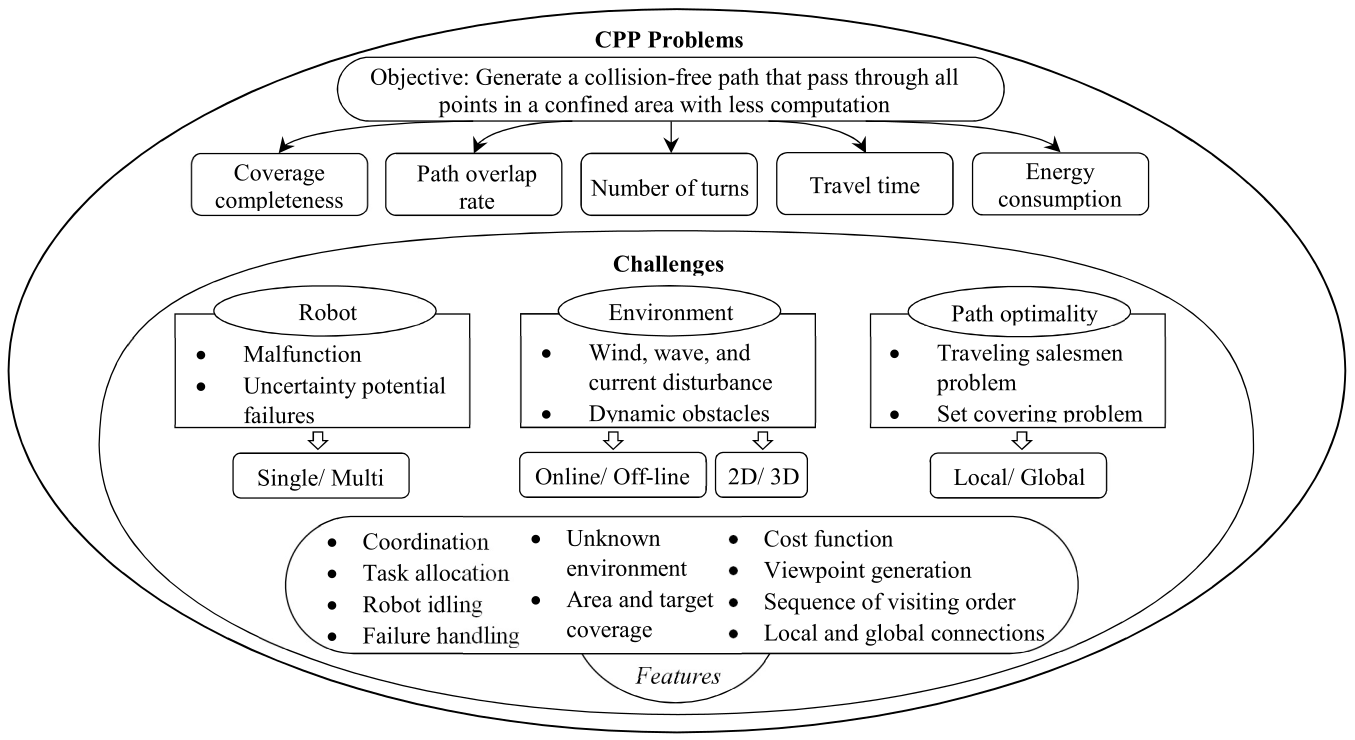
\includegraphics[width=\textwidth]{Images/general/overview_of_CPP.png}
    \caption{The objective and challenges in coverage path planning (CPP) problems.}
    \label{fig:overview_of_CPP}
\end{figure}

Over the years, researchers have developed a myriad of algorithms to address different aspects of path planning, ranging from basic algorithms to more advanced methodologies. CPP algorithms can be categorized into two approaches, classical algorithms, and heuristic-based algorithms. The summarized details of CPP algorithms according to the characteristics of the algorithms as stated in the paper \hyperlink{cite.main_review}{[2]} are classified as shown in (\autoref{fig:classifications_of_CPP}). 

\begin{figure}[htbp]
    \centering
    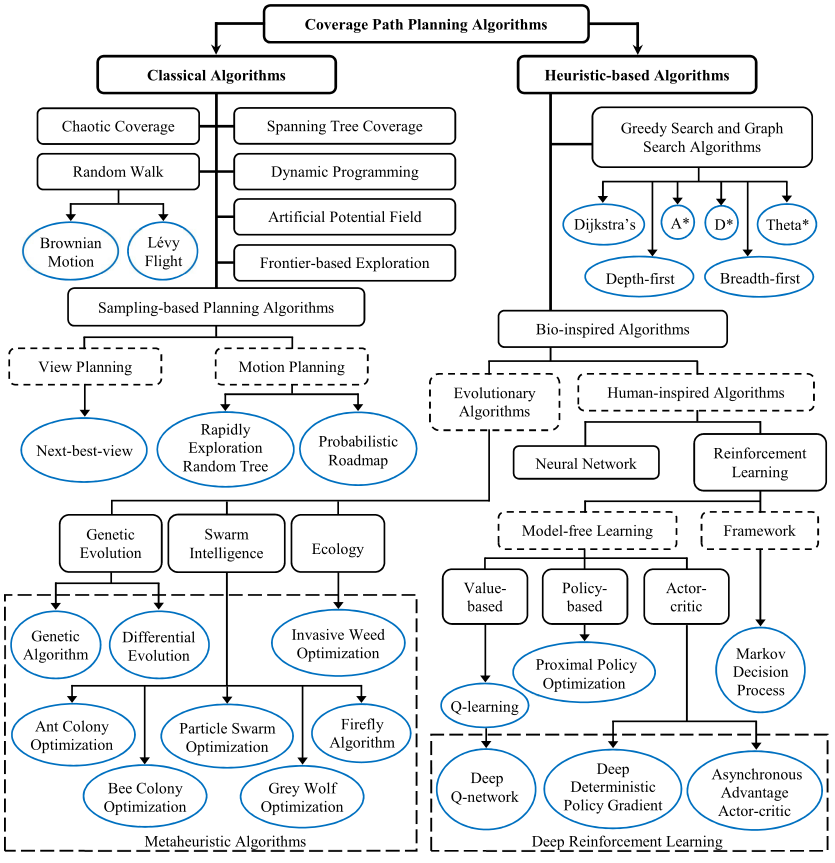
\includegraphics[height=22cm, width=\textwidth]{Images/general/general_classification.png}
    \caption{The classification of coverage path planning (CPP) algorithms.}
    \label{fig:classifications_of_CPP}
\end{figure}

\vspace{3mm}

Several algorithms relevant to coverage path planning for points or regions, which adhere to non-holonomic constraints with the objective of minimizing total route length, computational time, and energy consumption, are discussed below.


\subsection{Dubin's Path}

In the realm of geometric analysis and constrained path planning, the pioneering work of L.E. Dubins stands as a cornerstone, providing profound insights into the properties and characteristics of paths subject to curvature constraints. Dubins' seminal exploration, outlined in the paper \hyperlink{cite.dubins}{[1]}, lays a robust foundation for understanding the fundamental principles governing constrained path planning and provides critical insights into the properties of paths constrained by curvature.

\vspace{3mm}

At the core of Dubins' research lies the concept of R-geodesics, representing paths of minimal length under specified curvature constraints. This notion encapsulates the geometric essence of constrained paths, defining them as combinations of straight lines and circular arcs with a minimum radius of curvature, denoted as R. Dubins' theorem regarding the structure of R-geodesics in two dimensions provides a clear geometric understanding, asserting that such paths consist of no more than three segments, each comprising either a straight line or an arc of a circle with radius R. This theorem delineates the structure of minimal paths and imposes precise constraints on their composition, revealing the inherent simplicity of paths subject to curvature constraints.

\vspace{3mm}

Dubins rigorously proved the existence of R-geodesics using mathematical tools like Ascoli's theorem and concepts from E. Schmidt's proof of A. Schur's Lemma. These proofs confirm the theoretical existence of such paths and illuminate their analytical and geometric properties.

\vspace{3mm}

Dubins' work represents a significant milestone in the study of geometric analysis and constrained path planning, providing not only a solution to a specific geometric problem but also a methodological framework applicable to a broader class of problems in path planning and optimization. Therefore, many extensions of Dubins have been studied since then, integrating with other approaches to solve complex path planning problems. Due to its effectiveness towards curvature constraints and path length minimization, the Dubins path serves as a potential technique to inspire and inform further research into path planning algorithms for agricultural robots.


\subsection{Reeds-Shepp Paths}

Reeds-Shepp paths, introduced by J.A. Reeds and L.A. Shepp in the paper \hyperlink{cite.reeds}{[3]}, offers a flexible solution to optimal path planning for vehicles capable of moving forwards and backwards. Unlike Dubins paths, which only accommodate forward movement, Reeds-Shepp paths enhance maneuverability by incorporating reverse movements, doubling the range of possible maneuvers. This flexibility enables efficient navigation in complex environments, making them ideal for applications like robotics and autonomous vehicle navigation.

\vspace{3mm}

In agricultural robotics, Reeds-Shepp paths are particularly beneficial for tasks like weed removal, where precise navigation is essential. Their flexibility allows for efficient navigation through narrow spaces and around obstacles, reducing time and energy consumption. Reeds and Shepp's comprehensive analysis of Reeds-Shepp paths laid the foundation for subsequent research in optimal control and path planning, emphasizing the importance of considering a vehicle's full range of capabilities.





\subsection{Travelling Salesman Problem (TSP) with Neighborhoods} 

The Traveling Salesman Problem (TSP) represents a classic conundrum in optimization, challenging researchers to find the most efficient route for a salesman to visit a set of locations and return to the starting point while minimizing the total distance traveled. Renowned for its computational complexity and practical applications in logistics and route planning, the TSP has spurred numerous investigations into variants that more accurately reflect real-world scenarios.

\vspace{3mm}

One such variant, explored in the paper \hyperlink{cite.TSPN}{[4]}, introduces the concept of TSP with neighborhoods (TSPN). In this formulation, destinations are not singular points but rather areas or neighborhoods, complicating the problem by requiring the salesman to visit each neighborhood at least once without specifying exact points for each visit. TSPN is particularly relevant as it mirrors the challenge of navigating through regions (fields with weeds) rather than fixed points.

\vspace{3mm}

To address the challenges posed by TSPN, the paper introduces innovative approximation algorithms tailored to different types of neighborhoods, such as line segments or complex shapes described as "fat" regions. A notable contribution is the development of a constant factor approximation algorithm for neighborhoods represented as line segments, signifying a significant advancement in the field of geometric optimization.

\vspace{3mm}

A significant contribution of the paper is the m-guillotine method, which recursively subdivides the plane to approach a near-optimal solution. This method, along with key theoretical insights, underpins the algorithms' effectiveness in solving TSPN. However, it is essential to note that the TSPN problem is NP-hard, and the proposed algorithms provide only approximation solutions. While TSPN works with regions instead of points and strives to find the optimal solution, it does not explicitly consider the curvature constraints inherent in robotic path planning scenarios.











\subsection{Traveling Salesperson Problems for Dubins’ vehicle.}



After TSPN evolved from TSP, the challenges associated with optimal path planning for Dubins' vehicles, constrained by their minimum turning radius, have garnered significant attention. The paper \hyperlink{cite.TSP_with_dubins}{[5]} offers a thorough examination of these challenges and introduces innovative methodologies to overcome them.

\vspace{3mm}


At the core of this paper are two fundamental problems: the point-to-point shortest path problem (PTP) and the traveling salesperson problem (TSP) tailored for Dubins’ vehicles. These problems are crucial for developing algorithms capable of computing optimal or near-optimal paths for vehicles subject to nonholonomic constraints. the paper tackles the traveling salesperson problem (TSP) for Dubins’ vehicles, wherein the vehicle must visit a predefined set of locations in the most efficient route without revisiting any point. Acknowledging the computational complexity of exact solutions for larger point sets, the authors explore heuristic and approximation algorithms to efficiently approximate solutions.

\vspace{3mm}

The methodology outlined in the paper integrates rigorous mathematical frameworks and computational geometry to address the complexities of path planning for Dubins’ vehicles. By synthesizing Dubins constraints with the Traveling Salesperson Problem (TSP), the study offers a cohesive approach that bridges theoretical insights with practical solutions. this paper constitutes a significant contribution to the literature on path planning for nonholonomically constrained vehicles, paving the way for further advancements in navigating Dubins’ vehicles efficiently and effectively.











\subsection{Dubins Traveling Salesman Problem with Neighborhoods}

To address the challenges posed by regions in the Dubins Traveling Salesman Problem (DTSP), the paper \hyperlink{cite.DTSPN}{[6]} introduces a tailored formulation termed the Dubins Touring Regions Problem (DTRP). This novel approach aims to determine an optimal sequence of configurations for entering and exiting regions, all while minimizing the total path length. Unlike the conventional Traveling Salesman Problem (TSP), which focuses on finding the shortest route visiting a set of points, the DTSPN involves regions or neighborhoods, necessitating the vehicle to access each region at least once. This problem holds significant relevance in various applications, including autonomous drone surveillance, delivery systems, and robotic exploration, where vehicles must efficiently traverse specified areas while adhering to nonholonomic constraints.

\vspace{3mm}

The proposed algorithm for solving the DTRP leverages local iterative optimization techniques, taking into account the unique dynamics of Dubins vehicles. It begins with an initial sequence of region visits derived from solving an Euclidean TSP (ETSP), which serves as a proxy for the region centers. The algorithm then iteratively refines the entry and exit configurations to minimize the total tour length.

\vspace{3mm}

A key aspect of the solution method is its decoupled approach, optimizing the heading and position of each entry point independently. This simplification, facilitated by mathematical techniques that project the problem into a more manageable form, allows for efficient local optimization. The algorithm iterates until no further improvements can be made or a termination criterion is met, incorporating strategies to escape local minima by adjusting vehicle headings and repositioning at region boundaries.

\vspace{3mm}

Empirical validation of the algorithm demonstrates its effectiveness and efficiency across various scenarios, including different region shapes and configurations, particularly in dense environments where regions are close together. Comparative analysis against existing evolutionary algorithms showcases the proposed method's ability to produce high-quality solutions with significantly reduced computational time, making it suitable for real-time applications on modest hardware, such as onboard computers in UAVs.

\vspace{3mm}

Despite its capability to generate near-optimal paths while adhering to the non-holonomic constraints, the algorithm exhibits notable drawbacks in terms of computational efficiency. For instance, computing a near-optimal path for 30 regions may require over a minute, and the algorithm's performance further deteriorates with an increasing number of points, especially when they are closely positioned. Moreover, the algorithm's limitation in considering the overlap of regions represents a critical drawback, as it fails to account for this aspect in real-world scenarios, thereby impacting the path planning accuracy and efficiency.




\subsection{DTSPN with Overlappped Regions}



The paper \hyperlink{cite.overlap}{[7]} introduces the Intersecting Regions Algorithm (IRA) to address the challenges posed by intersecting regions in DTSPN. By explicitly considering the overlap among regions, IRA offers a more comprehensive solution compared to traditional methods. It leverages sampling within intersecting regions to construct feasible tours for autonomous vehicles, resulting in optimized route selection and more efficient path planning.

\vspace{3mm}

Furthermore, IRA reduces the computational complexity associated with path planning by adopting a polynomially scalable algorithmic structure. This scalability ensures IRA's viability even in scenarios with numerous regions of interest, where computational resources are limited. Monte Carlo simulations validate IRA's practical utility, showcasing significant performance enhancements, particularly in scenarios with high degrees of region overlap. However, despite its advancements, IRA still encounters challenges when dealing with a large number of points and close proximity points. These limitations highlight avenues for further research and development to enhance the algorithm's robustness and efficiency in addressing complex DTSPN scenarios.








\subsection{Path planning in confined spaces}


Navigating narrow and complex environments presents challenges for non-holonomic vehicles. In the paper \hyperlink{cite.mapping}{[8]}, the authors propose a path planning method tailored to address these challenges, focusing on generating paths with continuous curvature to ensure smooth operation in confined spaces.

\vspace{3mm}

The proposed method adopts a two-phase planning approach combining global and local strategies for efficient navigation. In the first phase, the authors employ the RTR (Rotate-Translate-Rotate) planner, a variation of the Rapidly Exploring Random Tree (RRT) method. This planner generates paths consisting of straight movements and in-place turning, simplifying complex maneuvering for navigating constrained spaces.

\vspace{3mm}

In the second phase, the global path is refined using the TTS local planning procedure. This planner approximates the initial path with a sequence of paths adhering to the vehicle's curvature constraints, ensuring smooth and feasible trajectories. The TTS planner can generate paths with continuous curvature turns (CC-turns) and straight segments, offering flexibility adaptable to various environmental constraints.

\vspace{3mm}

The paper also emphasizes maintaining similarity between global and local trajectories to avoid sudden changes in the path and ensure smooth passage through narrow regions. Ultimately, the objective is to enhance the capabilities of autonomous vehicles to operate safely and efficiently in diverse scenarios, thereby improving their practicality for everyday use.


\newpage

\section{Experimental Setup}

\subsection{Environment}
The environment for our coverage motion planning algorithm is situated in a grass field characterized by small grass uniformly distributed across the area. The grass field is representative of typical agricultural settings, where weed management is essential for maintaining crop quality and productivity. As the grass matures, it is common for various unwanted plants, particularly weeds, to grow sporadically throughout the field. Our primary focus in this study is on the removal of Rumex (commonly known as dock weeds), which pose a significant challenge to farmers. However, the algorithm can be adapted to target other types of weeds based on specific requirements, the only that change would be the detection system to identify the target weed.

\subsection{Importance of Weed Removal}
Importance of Weed Removal
We are concentrating on Rumex plants due to their detrimental impact on agricultural productivity and livestock health. Although Rumex plants are not inherently toxic, their presence in cattle feed can adversely affect the quality of milk production. Ensuring the purity of grass fed to cattle is crucial for producing high-quality, bio milk, which is not only more beneficial for human consumption but also promotes better health and well-being of the cattle. Pure grass feed leads to higher nutritional value in milk, contributing to improved dairy products. Therefore, effective weed management, particularly the removal of Rumex plants, is essential for maintaining the quality and productivity of grass fields.


\vspace*{6mm} 


Traditionally, farmers have resorted to manually removing these weeds, a labor-intensive and time-consuming process. Manual removal becomes particularly arduous in large fields, imposing significant physical strain on farmers and limiting the efficiency of weed management. Automating this process with robotic systems offers a promising solution to enhance agricultural practices and improve farmers' quality of life.

\vspace*{6mm}

\subsection{The Robot}

\subsubsection{Overview}

To efficiently remove weeds from the grass field, we employ a robust, four-wheeled robot specifically designed for this task. This section provides an in-depth look at the robot's external and internal features, highlighting the components that enable it to navigate the field and execute precise weed extraction.

\subsubsection{External Features}

The robot features a four-wheeled design, ensuring stability and effective maneuverability across uneven terrain. The choice of a four-wheeled configuration is crucial as it supports the internal weed extraction system, which occupies most of the internal space. The wheels are equipped with treads suitable for grass fields, providing the necessary traction and mobility.

\vspace*{6mm}

\textbf{Localization and Orientation:} For accurate positioning and orientation in the open field, the robot is equipped with two Real-Time Kinematic (RTK) GPS systems. RTK GPS technology is ideal for this environment, offering centimeter-level accuracy in localization, which is essential for precise navigation and weed targeting.

\vspace*{6mm}


\textbf{Vision System:} The robot incorporates two strategically placed cameras. The front-facing camera is oriented towards the ground, scanning for weeds ahead of the robot. This early detection allows the local planner to adjust the robot's path accordingly, ensuring efficient navigation and weed targeting. The second camera is mounted at the bottom center of the robot, directly above the extraction mechanism. This camera provides an accurate view of the weed's position beneath the robot, facilitating precise extraction.


\subsubsection{Internal Features}

The internal mechanism of the robot is crucial for the precise and efficient removal of weeds. It comprises several key components: a processing unit, a battery system, and the main weed extraction system.


\vspace*{6mm}


\textbf{Processing Unit: } The processing unit serves as the brain of the robot, orchestrating the various functions and ensuring smooth operation. It processes data from the cameras and GPS systems, making real-time decisions to control the navigation and extraction processes. The unit is equipped with advanced algorithms for path planning, weed detection, and tool control, enabling the robot to perform its tasks autonomously and efficiently.


\vspace*{6mm}

\textbf{Battery System: }
The robot is powered by a robust battery system designed to provide sufficient energy for extended field operations. The battery pack is engineered for easy replacement, ensuring minimal downtime and continuous operation. This power system supports all onboard electronics, including the processing unit, cameras, GPS, and the weed extraction mechanism.


\vspace*{6mm}


\textbf{Weed Extraction System: }
The heart of the weed removal process is the weed extraction system, inspired by CNC machine technology. This system features two moving rails that allow the internal extraction mechanism to move in both the x and y directions. Controlled by the processing unit, these rails provide precise positioning capabilities. The extraction mechanism can move approximately 60 cm in both the x and y directions, covering a significant area beneath the robot. Once a weed is detected, the system moves the tool directly above the weed. The mechanical tool is then lowered in the negative z direction to engage the weed.

\vspace*{6mm}

The extraction tool is designed with sharp implements and rotates at high speed to destroy the weed effectively. This rotation ensures that the weed is thoroughly eradicated and cannot regrow. After destroying the weed, the remnants are left on the field, eliminating the need to carry them, which would otherwise burden the robot. The robot’s internal system, with its 60 cm movement range in both directions, allows for efficient navigation. Each detected weed point can be associated with a circular region within which the robot can maneuver to remove the weed. This approach not only aids in accurate weed extraction but also facilitates efficient path planning. By considering these regions, the planning algorithm can optimize the robot's path to cover all weed points effectively.

\vspace*{6mm}

\textbf{Adaptive Regions and Uncertainty Management: }
The regions around each weed point also serve to manage uncertainty in weed detection. If the position of a weed is detected with less accuracy, the associated region can be adjusted accordingly. A larger uncertainty reduces the size of the region to ensure the robot remains closer to the center, enhancing the likelihood of successful extraction. This adaptive approach allows the robot to handle variations in detection accuracy, maintaining high efficiency and precision in weed removal. The robot's internal features are meticulously designed to support the complex task of weed removal. The combination of precise movement capabilities, robust processing power, and adaptive region management ensures that the robot can effectively and efficiently eradicate weeds from the grass field.

\subsection{Constraints}

With a comprehensive understanding of the robot's capabilities and features, it is essential to delve into the constraints that arise due to its mechanical system and the nature of the field in which it operates. These constraints significantly influence the development of an effective motion planning algorithm.

\vspace*{6mm}

\textbf{Non-Holonomic Nature:}
The robot is equipped with four regular wheels, limiting its movement capabilities. Unlike holonomic robots, which can move in any direction, our robot cannot move sideways. It is constrained to forward and backward movements and must make turns to change its direction. This non-holonomic nature adds a layer of complexity to the motion planning algorithm, as it must account for the robot's inability to change its heading instantaneously.

\vspace*{6mm}

\textbf{Turning Radius:} The robot has a minimum turning radius of 2 meters, meaning it cannot make sharp turns. This constraint necessitates careful planning to ensure the robot can navigate around obstacles and reach all designated weed points without making turns that exceed its turning capabilities.

\vspace*{6mm}

\textbf{Speed Variations:} The robot's speed must be carefully regulated to prevent damage to the grass and ensure precise weed removal. When moving in a straight path, the robot operates at a velocity of 0.8 m/s. However, when making a turn, the velocity is reduced to 0.4 m/s to maintain the 2-meter turning radius. This adjustment helps in maintaining stability and accuracy during turns, which is critical for avoiding collateral damage to the grass and ensuring efficient weed extraction.

\vspace*{6mm}

\textbf{Kinematic Constraints:} Given its non-holonomic nature and the minimum turning radius, the robot cannot change its heading angle at a specific position. Instead, it requires a certain amount of space to turn and align itself in the desired direction. These kinematic constraints must be factored into the motion planning algorithm to ensure smooth and feasible navigation across the field.

\vspace*{6mm}

\textbf{Field Constraints:} The field is covered with grass and scattered weeds, particularly the rumex plants. The random distribution of weeds means the robot must navigate the entire field efficiently to locate and remove all weeds. The algorithm must account for this scattered distribution and plan paths that ensure comprehensive coverage without unnecessary overlaps.


\vspace*{6mm}



With a clear understanding of the robot's constraints, we can now proceed to develop a motion planning algorithm that leverages these constraints to ensure comprehensive and efficient weed removal. By integrating considerations for non-holonomic movement, adaptive speed control, optimized coverage, obstacle avoidance, and environmental adaptability, the algorithm will facilitate the robot's autonomous operation, making the weed removal process more efficient and reducing the burden on farmers. This strategic approach not only enhances the robot's performance but also contributes to maintaining the health of the grass and improving the overall quality of the field.

























\subsection{Remnants}


Benefits of Robotic Weed Removal
Deploying robots for weed removal in grass fields presents several advantages:

Increased Efficiency: Robots can operate continuously and systematically cover large areas, ensuring thorough removal of unwanted plants without fatigue.
Labor Savings: Automating weed removal reduces the need for manual labor, freeing farmers to focus on other essential tasks and reducing physical strain.
Precision: Advanced sensors and algorithms enable robots to identify and target specific weeds, minimizing damage to the surrounding grass and ensuring effective weed management.
Health Benefits: By eliminating the need for manual weed removal, farmers can avoid the physical exertion and potential health risks associated with prolonged exposure to outdoor conditions and repetitive movements.
Enhanced Livestock Health: Ensuring the purity of grass feed leads to healthier cattle, which in turn produce higher-quality milk, enhancing overall dairy production.


Experimental Objective
The primary objective of our experimental setup is to develop and validate a coverage motion planning algorithm that enables robots to efficiently navigate and manage weed removal in grass fields. By leveraging advanced robotic technology, we aim to automate the process of identifying and removing Rumex plants, ultimately improving agricultural productivity and promoting sustainable farming practices.

Methodology
The experimental setup involves the following key steps:

Field Analysis: Detailed mapping of the grass field to identify the distribution of grass and Rumex plants.
Algorithm Development: Creating a coverage motion planning algorithm tailored to navigate the field and target Rumex plants for removal.
Robotic Implementation: Equipping robots with necessary sensors and tools to detect and remove weeds, followed by field testing to ensure operational efficiency.
Performance Evaluation: Assessing the effectiveness of the robotic system in terms of coverage, weed removal accuracy, and operational efficiency.
By addressing the challenges of weed management through robotic automation, we aim to revolutionize agricultural practices, making farming more sustainable, efficient, and farmer-friendly. This innovative approach not only enhances the productivity of grass fields but also contributes to the overall well-being of livestock and farmers alike.
















Integrating Constraints into Motion Planning
Understanding the mechanical and field constraints is crucial for developing an effective coverage motion planning algorithm. These constraints guide the design of the algorithm to ensure it is practical and feasible under real-world conditions.

Path Planning with Non-Holonomic Constraints: The algorithm must plan paths that respect the robot's non-holonomic nature. This involves generating smooth, continuous paths that the robot can follow without needing to make sharp turns. Techniques such as Dubins curves, which are designed for non-holonomic vehicles, can be employed to create feasible paths that the robot can navigate.

Adaptive Speed Control: Incorporating variable speed control into the algorithm allows for safe and efficient navigation. The robot should move faster in straight paths to cover more ground quickly and slow down during turns to maintain stability and precision. This adaptive speed control also helps in preventing damage to the grass, ensuring that the robot's operations are minimally invasive.

Coverage Optimization: The algorithm should optimize the coverage pattern to ensure that all weeds are detected and removed efficiently. By considering the robot's 60 cm movement range in both directions, the algorithm can plan paths that cover larger areas without unnecessary backtracking. This optimization reduces the total time and energy required for weed removal.

Obstacle Avoidance and Navigation: The algorithm must include robust obstacle avoidance capabilities to navigate around natural terrain features and any unforeseen obstacles. This ensures the robot can continue its operation smoothly without interruptions.

Handling Environmental Variability: To ensure reliable performance under varying environmental conditions, the algorithm can incorporate sensor feedback to adjust the robot's path and speed in real-time. This adaptability enhances the robot's resilience and operational efficiency.
\newpage



\end{document}
